\section{Introduction}\label{sec:intro}
In this project we are given some basic volume visualization application and will implement several additional features in order to enhance this application. To be able to clearly explain the added functionality, we start by shortly describing the initial functioning of the application. Technically speaking, the application is not even a real raycaster, as it initially only takes a slice through the data, and projects the data that is found on this slice onto the viewing window (see figure \ref{fig:raycaster0}). The slice is defined in such a way that it always goes exactly through the center of the volume bounding box, and is oriented perpendicular to the view vector \texttt{viewVec} at all times. As the view vector is again perpendicular to the view window, the slice is always parallel to the view window. The width and height of the slice are both defined by the diagonal of the bounding box. This is an obvious choice, because this is the smallest dimension that ensures that no data can ever lie outside of the slice area. Looking at the code of the initial application we observe that all of the above is realized by a simple nested for-loop that walks along all the pixels in horizontal and vertical direction, and retrieves the value that is being found on the slice.

\begin{figure}[h!]
    \centering
    \captionsetup{justification=centering,margin=0.5cm}
    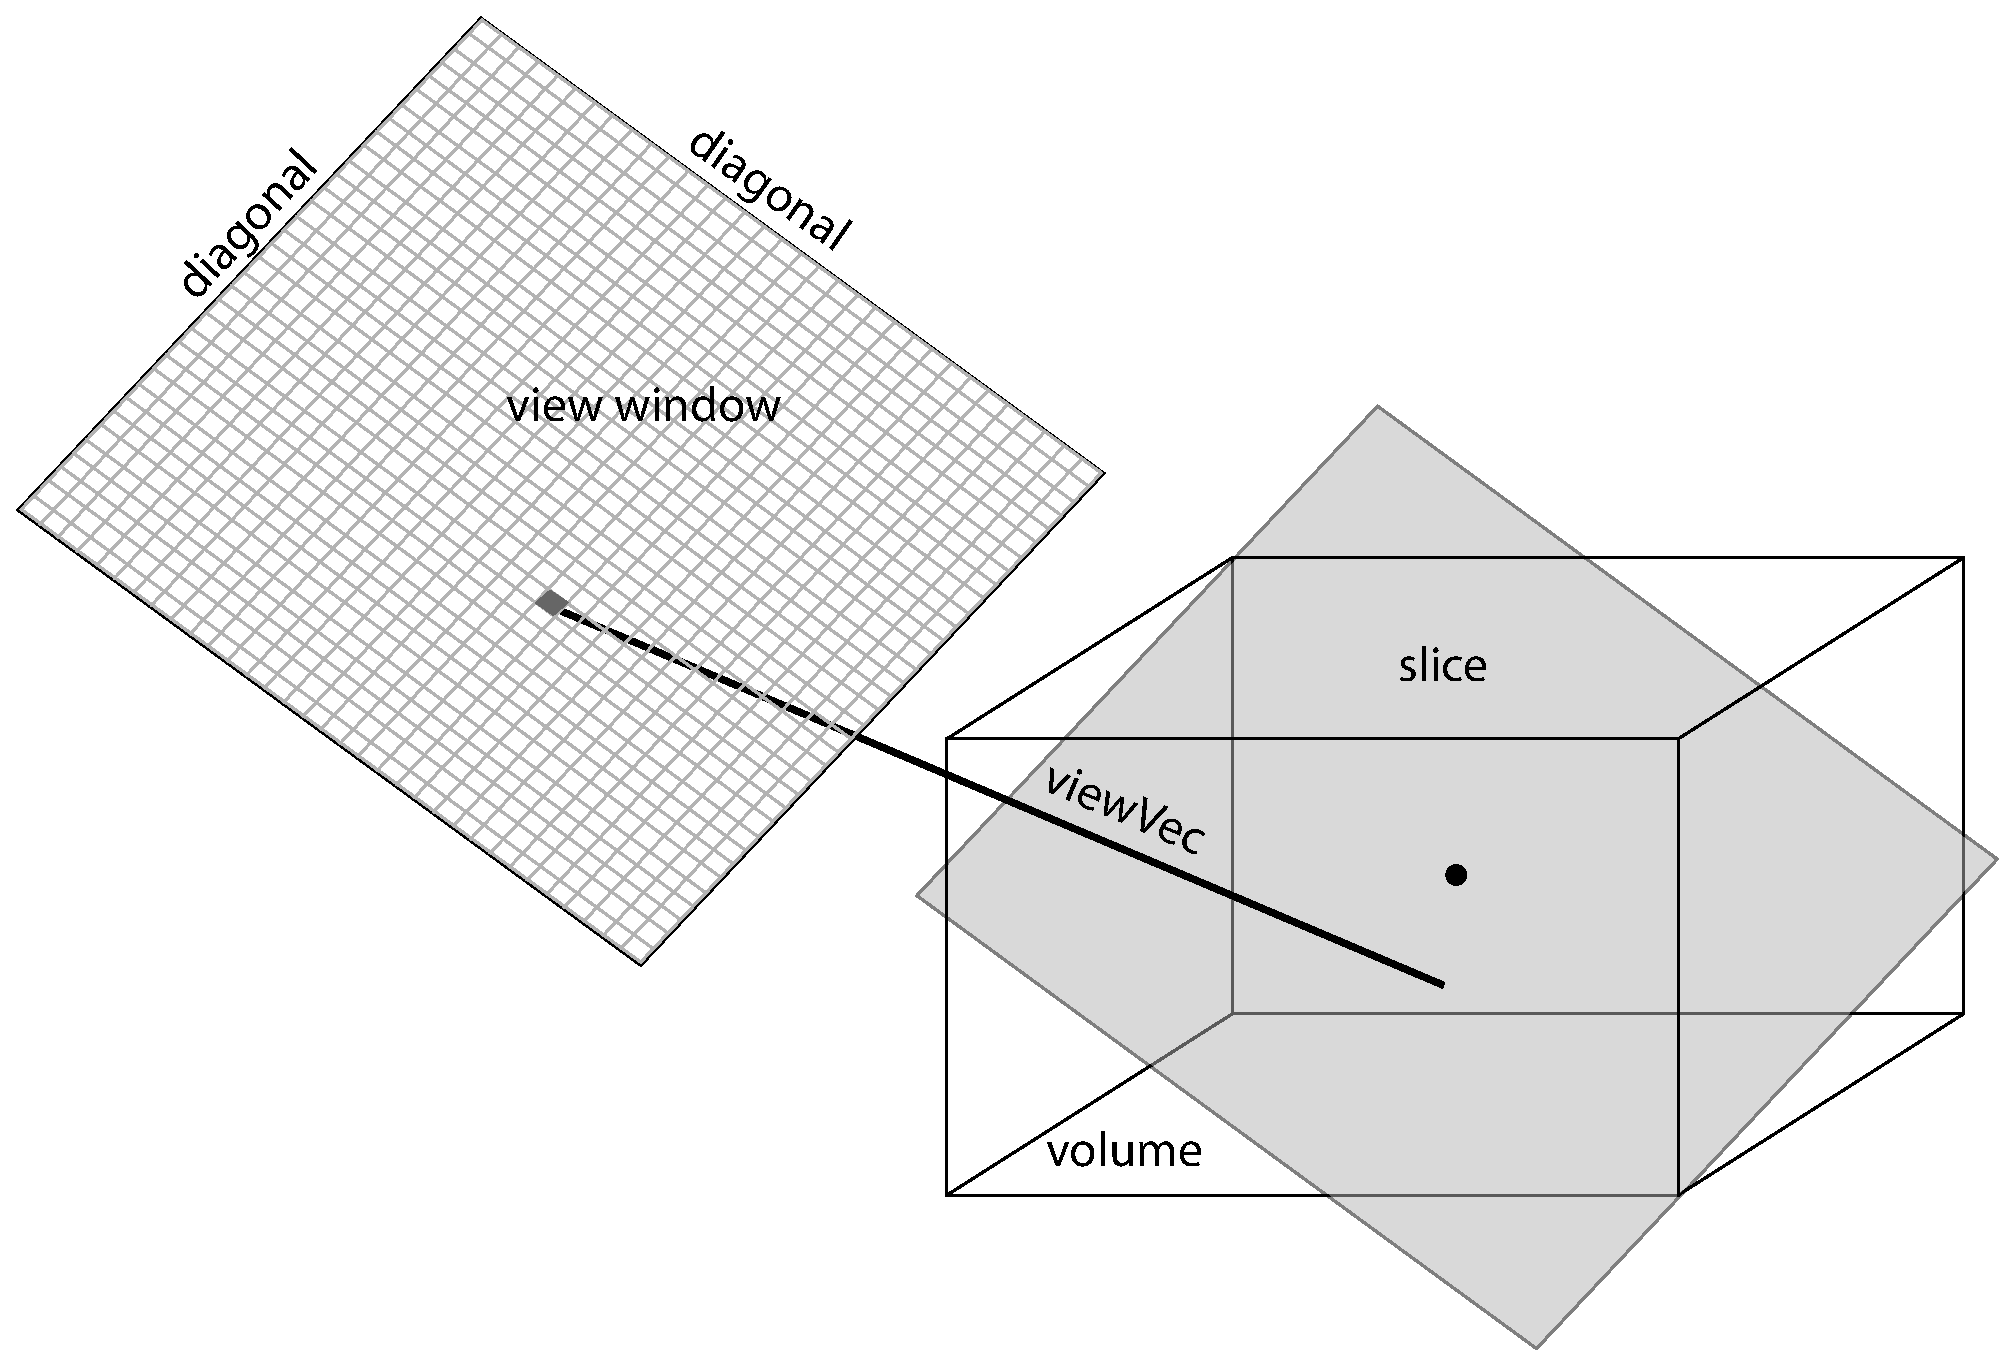
\includegraphics[width=0.8\textwidth]{img/raycaster0.pdf}
    \caption{The initial raycaster application: only a slice of the data within the volume is taken and projected onto the image (screen pixels)}
    \label{fig:raycaster0}
\end{figure}

With this application as a starting point, we devote the upcoming sections to explaining the additional features that were implemented. We start in section \ref{sec:mip} with the implementation of a Maximum Intensity Projection method. We furthermore adjust the interpolation technique for the points on a casted ray from a nearest neighbor interpolation to a tri-linear one. Because the implementation of a MIP greatly reduces the performance of the application, we present several performance enhancement methods in section \ref{subsec:perf_enh}. In section \ref{sec:compositing} we present an alternative implementation for the MIP, namely compositing. Section \ref{sec:opacity} finally describes how ...\todo{!}

